\documentclass[tikz]{standalone}

\begin{document}
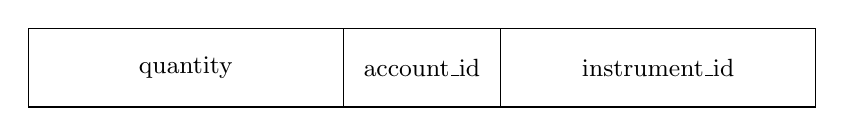
\begin{tikzpicture}[font=\small] % Using smaller font
    % Drawing the data block
    \draw (0,0) rectangle (10,1);
    % \node at (5,1.3) {Data Block for 'position' Message Format};

    % Divisions for each attribute
    \draw (0,0) -- (0,1); % start
    \draw (4,0) -- (4,1); % quantity 8 bytes
    \draw (6,0) -- (6,1); % account_id 4 bytes (present)
    \draw (10,0) -- (10,1); % instrument_id 8 bytes

    % Labels for each attribute, centered within their sub-cell
    \node at (2,0.5) {quantity};
    \node at (5,0.5) {account\_id};
    \node at (8,0.5) {instrument\_id};
\end{tikzpicture}
\end{document}
